% !TeX root = simplesnt-doc.tex
\documentclass{simplesnt}

%% Helpful packages
\usepackage{simplebnf}[2023/11/25]
\usepackage{kotex}
\usepackage{xcolor}
\usepackage{amsmath,amssymb}
\usepackage{amsfonts}
\usepackage{eso-pic}
\usepackage{tikz}
\usetikzlibrary{calc,positioning,fit,arrows.meta,backgrounds}
\usepackage{siunitx}
\usepackage{caption}
\usepackage{listings}
\usepackage{mathrsfs}
\usepackage{stmaryrd}
\usepackage{subcaption}
\usepackage{graphicx}
\usepackage{colortbl}


\captionsetup{font=small}
\lstset{basicstyle = \small\ttfamily, breaklines}

\usepackage{tabularray}
\UseTblrLibrary{booktabs}

\usepackage{metalogo}
\usepackage{kotex-logo}


\newcommand{\textalt}[2]{#1\textsubscript{\ensuremath{\text{\scriptsize\textit{#2}}}}}
\newcommand{\CILmm}{\texorpdfstring{CIL-\kern0.08em-}{CIL--}}
\newcommand{\fainttablerow}{\\[0.2ex]\arrayrulecolor{black!12}\hline\arrayrulecolor{black}}
\newcommand*{\presentfont}[1]{{\fontspec{#1}#1}}
\ExplSyntaxOn
\bool_if:nF { \sys_if_engine_xetex_p: || \sys_if_engine_luatex_p: }
  { \newcommand*{\fontspec}[1]{} }
\ExplSyntaxOff

\title{\CILmm{} 합성을 통한 Sparrow 분석기 공격}
\author{정원준}

\begin{document}
\date{2026년 7월 16일}
\maketitle


\begin{frame}
  \frametitle{목차}
  \tableofcontents
\end{frame}

\section{정적 분석기 공격}
\begin{frame}[c, fragile]
  \frametitle{정적 분석이란?}

  \setlength{\columnsep}{16pt}

  \begin{columns}[T,onlytextwidth]
    \column{0.46\textwidth}
    \hfill
    \begin{minipage}{0.78\linewidth}
    \lstset{
      language=Python,
      basicstyle=\ttfamily\small,
      lineskip=2pt,
      columns=fullflexible,
      escapeinside={(*@}{@*)},
    }
    \begin{lstlisting}
x = 1
while x < 10000:
    (*@\textcolor{red}{x = x + 1}@*)
print(x)
    \end{lstlisting}
    \end{minipage}

    \column{0.54\textwidth}
    \vspace{8pt}
    \begin{itemize}
      \item<2-> x가 어떤 값을 가질 수 있을까?
      \item<3-> x가 특정 위치에서 어떤 값을 가질 수 있을까?
      \item<4-> 프로그램을 돌려보지 않고 미리 알 수는 없을까?
      \item<5-> \textcolor{red}{완벽하게 알 수는 없음!}
      \item<6-> ``Rice's Theorem''
    \end{itemize}
  \end{columns}

\end{frame}
\begin{frame}[fragile]
  \frametitle{넓게 어림잡기}

  \begin{center}
    \begin{minipage}{0.34\linewidth}
      \begin{lstlisting}[basicstyle=\small\ttfamily, escapeinside={(*@}{@*)}]
if x > 0:
    x = 3
else:
    x = -3
(*@\texttt{print(x)}@*)
      \end{lstlisting}
    \end{minipage}
  \end{center}

  \vspace{12pt}

  \begin{center}
    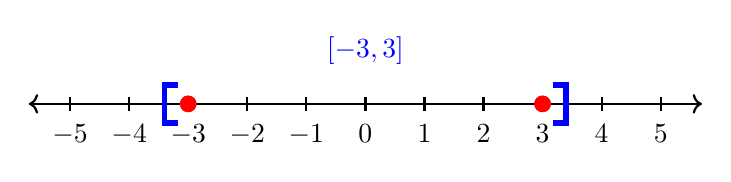
\begin{tikzpicture}[x=0.75cm, y=0.75cm]
      \draw[<->, thick] (-5.7,0) -- (5.7,0);
      \foreach \x in {-5,-4,...,5} {
        \draw[thick] (\x,0.12) -- (\x,-0.12);
        \node[below] at (\x,-0.18) {\(\x\)};
      }
      \only<2->{
        \fill[red] (-3,0) circle (3pt);
        \fill[red] (3,0) circle (3pt);
      }
      \uncover<3->{
        \draw[blue, line width=2pt]
          (-3.18,-0.32) -- (-3.4,-0.32) -- (-3.4,0.32) -- (-3.18,0.32);
        \draw[blue, line width=2pt]
          (3.18,-0.32) -- (3.4,-0.32) -- (3.4,0.32) -- (3.18,0.32);
        \node[blue, above] at (0,0.5) {\([ -3, 3 ]\)};
        \fill[red] (-3,0) circle (3pt);
        \fill[red] (3,0) circle (3pt);
      }
    \end{tikzpicture}
  \end{center}
\end{frame}

\begin{frame}[fragile]
  \frametitle{공격 프로그램의 예시}

  \begin{center}
    \begin{minipage}{0.34\linewidth}
      \begin{visibleenv}<2->
      \begin{lstlisting}[basicstyle=\small\ttfamily, escapeinside={(*@}{@*)}]
if x > 0:
    x = 3
else:
    x = -3
(*@\only<2>{\texttt{print(x)}}\only<3->{\textcolor{red}{\texttt{y = 10 / x}}}@*)
      \end{lstlisting}
      \end{visibleenv}
    \end{minipage}
    \makebox[0pt][l]{\hspace{16pt}\visible<3->{\textcolor{red}{false alarm 발생}}}
  \end{center}

  \vspace{12pt}

  \begin{visibleenv}<2->
    \begin{center}
      \begin{tikzpicture}[x=0.75cm, y=0.75cm]
        \draw[<->, thick] (-5.7,0) -- (5.7,0);
        \foreach \x in {-5,-4,...,5} {
          \draw[thick] (\x,0.12) -- (\x,-0.12);
          \node[below] at (\x,-0.18) {\(\x\)};
        }
        \fill[red] (-3,0) circle (3pt);
        \fill[red] (3,0) circle (3pt);
        \draw[blue, line width=2pt]
          (-3.18,-0.32) -- (-3.4,-0.32) -- (-3.4,0.32) -- (-3.18,0.32);
        \draw[blue, line width=2pt]
          (3.18,-0.32) -- (3.4,-0.32) -- (3.4,0.32) -- (3.18,0.32);
        \node[blue, above] at (0,0.5) {\([ -3, 3 ]\)};
        \fill[red] (-3,0) circle (3pt);
        \fill[red] (3,0) circle (3pt);
        \only<3->{
          \draw[red, line width=1.5pt] (0,0) circle (3pt);
        }
        \only<4->{
          \node[overlay, below] at (0,-1.0)
            {이런 공격을 일반적인 분석기에 대해서 하는 것이 목표};
        }
      \end{tikzpicture}
    \end{center}
  \end{visibleenv}
\end{frame}
\begin{frame}
  \frametitle{공격의 기대효과}
  \begin{itemize}
    \item<2-> 분석기의 약점을 파악하고 강화하는 가이드라인으로 사용
    \item<3-> 분석이 잘 안 되는 코드 조각을 삽입해서 난독화로 사용
  \end{itemize}
\end{frame}



\section{Sparrow 분석기 공격 목표}


\begin{frame}
  \frametitle{Sparrow 공격 목표}
  \begin{itemize}
    \uncover<1->{
      \item 정밀도 공격:
        \newline abstract semantics가 concrete semantics를 너무 크게 포함함
        \par
        \vspace{0.6em}
        \begin{center}
        \hspace*{-1.5em}
        \resizebox{0.9\textwidth}{!}{%
        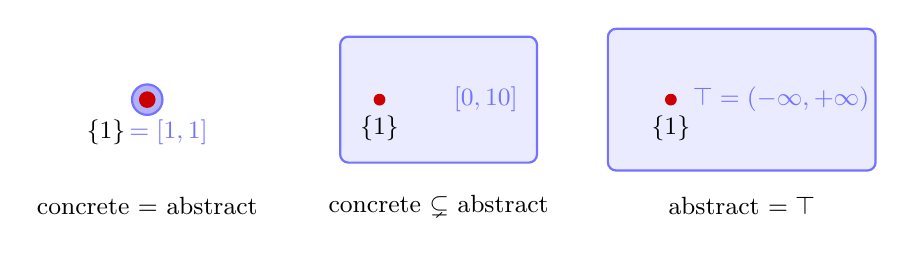
\begin{tikzpicture}[
            abset/.style={draw=blue!55, fill=blue!8, thick, rounded corners=3pt},
            conc/.style={circle, fill=red!80!black, inner sep=1.5pt},
            panelcap/.style={align=center, font=\small},
          ]
          % --- Panel 1: concrete = abstract (blue coincides with red point) ---
          \node[circle, draw=blue!55, fill=blue!30, thick, inner sep=0, minimum size=11pt] at (0,0) {};
          \node[circle, fill=red!80!black, inner sep=0, minimum size=6pt] at (0,0) {};
          \node[font=\small] at (0,-0.42) {$\{1\}$\,\textcolor{blue!55}{$=[1,1]$}};
          \node[panelcap] at (0,-1.35) {concrete $=$ abstract};

          % --- Panel 2: concrete < abstract (point & interval centered by box height) ---
          \begin{scope}[xshift=3.7cm]
            \draw[abset] (-1.25,-0.8) rectangle (1.25,0.8);
            \node[conc, label={[font=\small]below:$\{1\}$}] at (-0.75,0) {};
            \node[blue!55, font=\small] at (0.6,0) {$[0,10]$};
            \node[panelcap] at (0,-1.35) {concrete $\subsetneq$ abstract};
          \end{scope}

          % --- Panel 3: abstract = top (point & interval centered by box height) ---
          \begin{scope}[xshift=7.55cm]
            \draw[abset] (-1.7,-0.9) rectangle (1.7,0.9);
            \node[conc, label={[font=\small]below:$\{1\}$}] at (-0.9,0) {};
            \node[blue!55, font=\small] at (0.5,0) {$\top=(-\infty,+\infty)$};
            \node[panelcap] at (0,-1.35) {abstract $=\top$};
          \end{scope}
        \end{tikzpicture}}
        \end{center}
    }
    \vspace{0.4em}
    \uncover<2->{
      \item soundness 공격:
        \newline concrete semantics가 abstract semantics에 포함되지 않음(버그)
        \par\vspace{0.5em}
        \begin{center}
        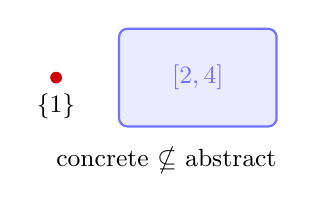
\begin{tikzpicture}[
            abset/.style={draw=blue!55, fill=blue!8, thick, rounded corners=3pt},
            conc/.style={circle, fill=red!80!black, inner sep=1.5pt},
            panelcap/.style={align=center, font=\small},
          ]
          \draw[abset] (-1.0,-0.62) rectangle (1.0,0.62);
          \node[blue!55, font=\small] at (0,0) {$[2,4]$};
          \node[conc, label={[font=\small]below:$\{1\}$}] at (-1.8,0) {};
          \node[panelcap] at (-0.4,-1.05) {concrete $\nsubseteq$ abstract};
        \end{tikzpicture}
        \end{center}
    }
  \end{itemize}
\end{frame}


\begin{frame}
  \frametitle{Sparrow의 기본 구조}
  \begin{center}
  \resizebox{0.88\textwidth}{!}{%
  \begin{tikzpicture}[
      codeblock/.style={draw=black!55, rounded corners=3pt, fill=black!5,
        align=left, font=\ttfamily\footnotesize, inner sep=6pt},
      cfgnode/.style={draw=blue!55, rounded corners=2pt, fill=blue!12,
        align=center, font=\ttfamily\footnotesize, inner sep=4pt, minimum width=2.1cm},
      graybox/.style={draw=black!55, rounded corners=3pt, fill=black!4, inner sep=11pt},
      procbox/.style={draw=red!55, rounded corners=4pt, fill=red!10, very thick,
        align=center, font=\Large\bfseries, inner sep=8pt},
      blabel/.style={font=\large\bfseries, black!80},
      flow/.style={-{Stealth[length=3mm]}, very thick, black!70},
      elbl/.style={font=\normalsize, black!75},
    ]
    \useasboundingbox (-1.7,-6.3) rectangle (12.1,2.85);
    % --- top row: C, CIL, CFG (centers aligned at y=0) ---
    \node<1->[codeblock] (c) at (0,0) {%
      int main() \{\\
      \ \ int x = 1;\\
      \ \ if (x == 1) \{\\
      \ \ \ \ x++;\\
      \ \ \}\\
      \ \ return x;\\
      \}};
    \node<2->[codeblock] (cil) at (4.7,0) {%
      int main(void) \{\\
      \ \ int x;\\
      \ \ x = 1;\\
      \ \ if (x == 1) \{\\
      \ \ \ \ x = x + 1;\\
      \ \ \}\\
      \ \ return x;\\
      \}};
    % CFG nodes (stacked, explicit coords)
    \node<3->[cfgnode] (n0) at (9.4, 1.5)  {x = 1};
    \node<3->[cfgnode] (n1) at (9.4, 0.5)  {x == 1 ?};
    \node<3->[cfgnode] (n2) at (9.4,-0.5)  {x = x + 1};
    \node<3->[cfgnode] (n3) at (9.4,-1.5)  {return x};
    \draw<3->[flow] (n0) -- (n1);
    \draw<3->[flow] (n1) -- (n2) node[elbl, midway, right=1pt]{T};
    \draw<3->[flow] (n2) -- (n3);
    \coordinate (fr) at (11.35,-0.5);
    \draw<3->[flow] (n1.east) .. controls +(0.85,0) and +(0.85,0) .. (n3.east)
      node[elbl, pos=0.5, right=1pt]{F};
    \begin{scope}[on background layer]
      \node<3->[graybox, fit=(n0)(n3)(fr)] (cfg) {};
    \end{scope}

    % --- names above each box ---
    \node<1->[blabel] at (0,2.35)   {C};
    \node<2->[blabel] at (4.7,2.35)  {CIL};
    \node<3->[blabel] at (9.4,2.35)  {CFG};

    % --- horizontal arrows in the row ---
    \draw<2->[flow] (c.east)   -- (cil.west);
    \draw<3->[flow] (cil.east) -- (cfg.west);

    % --- Sparrow (lower layer, large) receives CFG as input ---
    \node<4->[procbox, minimum width=10cm, minimum height=1.5cm] (sp) at (5.0,-4.2)
      {Sparrow\\[2pt]{\normalsize (정적분석)}};
    \draw<4->[flow] (cfg.south) -- (cfg.south |- sp.north)
      node[elbl, midway, left=2pt, font=\fontsize{15}{15}\selectfont]{입력};

    % --- Sparrow output: downward arrow labelled "분석 결과" ---
    \draw<5->[flow] (sp.south) -- ++(0,-1.05)
      node[midway, right=4pt, font=\fontsize{15}{15}\selectfont, text=black!80]{분석 결과};
  \end{tikzpicture}}
  \end{center}
\end{frame}


\section{\CILmm{} 언어}

\begin{frame}
  \frametitle{CIL 언어}
  \begin{center}
  \resizebox{0.68\textwidth}{!}{%
  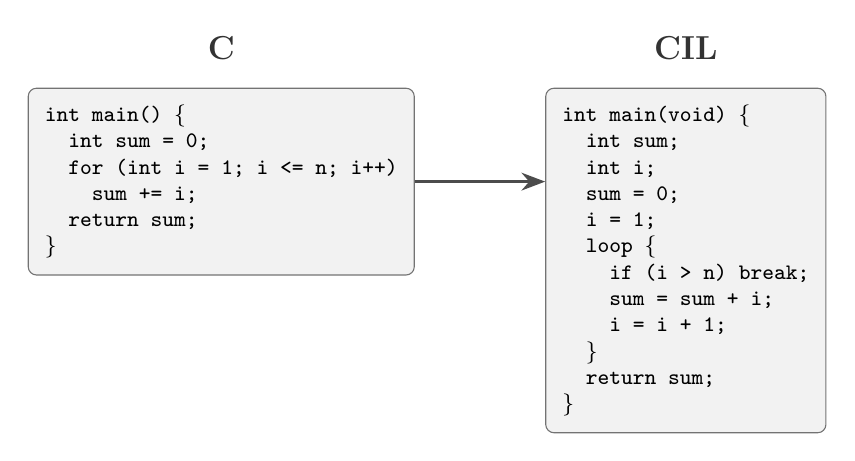
\begin{tikzpicture}[
      codeblock/.style={draw=black!55, rounded corners=3pt, fill=black!5,
        align=left, font=\ttfamily\footnotesize, inner sep=6pt},
      blabel/.style={font=\large\bfseries, black!80},
      flow/.style={-{Stealth[length=3mm]}, very thick, black!70},
    ]
    \node[codeblock, anchor=north] (c) at (0,0) {%
      int main() \{\\
      \ \ int sum = 0;\\
      \ \ for (int i = 1; i <= n; i++)\\
      \ \ \ \ sum += i;\\
      \ \ return sum;\\
      \}};
    \node[codeblock, anchor=north] (cil) at (5.9,0) {%
      int main(void) \{\\
      \ \ int sum;\\
      \ \ int i;\\
      \ \ sum = 0;\\
      \ \ i = 1;\\
      \ \ loop \{\\
      \ \ \ \ if (i > n) break;\\
      \ \ \ \ sum = sum + i;\\
      \ \ \ \ i = i + 1;\\
      \ \ \}\\
      \ \ return sum;\\
      \}};
    \node[blabel] at (0,0.5)    {C};
    \node[blabel] at (5.9,0.5)  {CIL};
    \draw[flow] (c.east) -- (c.east -| cil.west);
  \end{tikzpicture}}
  \end{center}
  \vspace{0.4em}
  \begin{itemize}
    \item<1-> C의 부분집합 --- 분석을 쉽게 할 수 있는 언어
    \item<2-> side effect 제거 
    \item<3-> 함수 호출은 그 자체로 한 statement
    \item<4-> $\cdots$
  \end{itemize}
\end{frame}

\begin{frame}
  \frametitle{\CILmm{} 언어}
  \begin{itemize}
    \item<1-> completeness 공격: 튜링 완전한 subset이기만 하면 충분 (Rice Theorem 덕분)
    \item<2-> soundness 공격: feature가 많을수록 좋음 (버그를 찾는 것이므로)
    \item<3-> CIL- : 의미적으로 관심 없는 것 제거 --- 확장 계획도 없음 (typedef, struct 등)
    \item<4-> \CILmm{} : 일단 미니멀하게 만들기 위해 이것저것 제거 --- 나중에 추가 희망 (포인터·malloc/free, 배열, int 외 타입)
  \end{itemize}
\end{frame}

\section{Sparrow의 실행의미와 대응시키기}

\begin{frame}
  \frametitle{실행의미가 잘 정의되는가?}

  \begin{itemize}
    \item<1-> 가장 큰 문제: Sparrow는 concrete semantics를 정확히 정의하지 않음
      \begin{itemize}
        \item<2-> C: ISO C 표준이 있지만 자연어로 되어 있어서 엄밀하진 않음
        \item<3-> CIL: 마찬가지로 엄밀한 실행의미가 없음
        \item<4-> Sparrow: 아예 없음
        \item<5-> 공격기: \CILmm{}에 대한 big-step 나무구조와 증명 생성기는 있음
      \end{itemize}
    \item<6-> 그렇다면, 공격기의 concrete 실행의미가 Sparrow의 abstract 실행의미에
      포함되지 않을 때 ``soundness가 깨졌다''고 말할 수 있는가?
    \item<7-> 각종 비결정성을 모두 제거해야 제대로 공격 가능
  \end{itemize}
\end{frame}


\begin{frame}
  \frametitle{비결정성을 제거하지 않으면...}
  
  \begin{itemize}
    \item<1-> 공격을 성공했다고 생각했는데...
                  \begin{center}
      \begin{tikzpicture}[
          abset/.style={draw=blue!55, fill=blue!8, thick, rounded corners=2pt},
          conc/.style={circle, fill=red!80!black, inner sep=1.4pt},
        ]
        \useasboundingbox (-0.3,-1.15) rectangle (7.9,0.85);
        \draw[abset] (0,-0.65) rectangle (1.5,0.65);
        \node[blue!55, font=\scriptsize] at (0.75,0.35) {abstract};
        \node[conc] at (3.0,0) {};
        \node[font=\scriptsize, anchor=base] at (3.0,-0.95) {concrete};
        \node[font=\small, right] at (3.5,0) {$\Rightarrow$ soundness 깨짐 (공격 성공!)};
      \end{tikzpicture}
      \end{center}
    \item<2-> 사실 그건 비결정성 때문이었다고?!
                              \begin{center}
      \begin{tikzpicture}[
          abset/.style={draw=blue!55, fill=blue!8, thick, rounded corners=2pt},
          conc/.style={circle, fill=red!80!black, inner sep=1.4pt},
        ]
        \useasboundingbox (-0.3,-1.15) rectangle (7.9,0.85);
        \draw[abset] (0,-0.65) rectangle (1.5,0.65);
        \node[blue!55, font=\scriptsize] at (0.75,0.35) {abstract};
        \node[conc] at (0.75,0) {};
        \node[conc] at (3.0,0) {};
        \node[font=\scriptsize, anchor=base] at (0.75,-0.95) {Sparrow-concrete};
        \node[font=\scriptsize, anchor=base] at (3.0,-0.95) {Attack-concrete};
        \node[font=\small, right] at (3.5,0) {$\Rightarrow$ soundness 깨지지 않음.};
      \end{tikzpicture}
      \end{center}
    \item<3-> 따라서 모든 비결정성을 제거해야 올바른 공격을 할 수 있다.
  \end{itemize}
\end{frame}


\begin{frame}
  \frametitle{C 언어의 비결정성}

  {\scriptsize
  \centering
  \setlength{\tabcolsep}{2.0pt}
  \renewcommand{\arraystretch}{1.08}
  \begin{tabular}{@{}p{0.24\linewidth}p{0.31\linewidth}p{0.28\linewidth}p{0.16\linewidth}@{}}
    \toprule
    \textbf{예} & \textbf{C} & \textbf{CIL} & \textbf{\CILmm{}} \\
    \midrule
    \texttt{h(f(),g())} \newline \texttt{f()+g()} \newline \texttt{\{f(),g()\}} & 계산 순서 비결정 & 함수 호출은 expression으로 들어가지 않음 & OK \fainttablerow
    \texttt{sizeof(int (*)[n++])} & \texttt{n++}을 실행하거나/하지 않거나 & \texttt{n++} 문법이 없음 & OK \fainttablerow
    \texttt{i = i++ + 1;} & Undefined Behavior & \texttt{i++} 문법이 없음 & OK \fainttablerow
    \texttt{int x; use(x);} & indeterminate value & indeterminate value & 합성 시 생성 x\fainttablerow
    \texttt{"a" == "a"} & true/false 모두 가능 & 여전히 비결정적 & string 없음 \fainttablerow
    \texttt{char c = -1;} & -1/255 & 여전히 비결정적 & char 없음 \fainttablerow
    \texttt{x >> 1} & \texttt{x} $< 0$ 일 때 UB & 여전히 비결정적 & 비트연산 없음 \fainttablerow
    \texttt{malloc(n)} & 메모리 주소가 비결정적 & fresh object & 포인터 없음 \\
    \bottomrule
  \end{tabular}
  }

  \uncover<2->{
    이외에도 malloc 실패 여부, struct의 byte 패딩, signed 정수 overflow 등 여러 가지 고려해야 할 비결정성이 많음
  }
\end{frame}

\section{메모리를 포함하여 합성하는 방법}

\begin{frame}
  \frametitle{증명나무 합성과 메모리}
  \begin{overlayarea}{\textwidth}{0.72\textheight}
    \only<1>{\noindent\makebox[\textwidth][c]{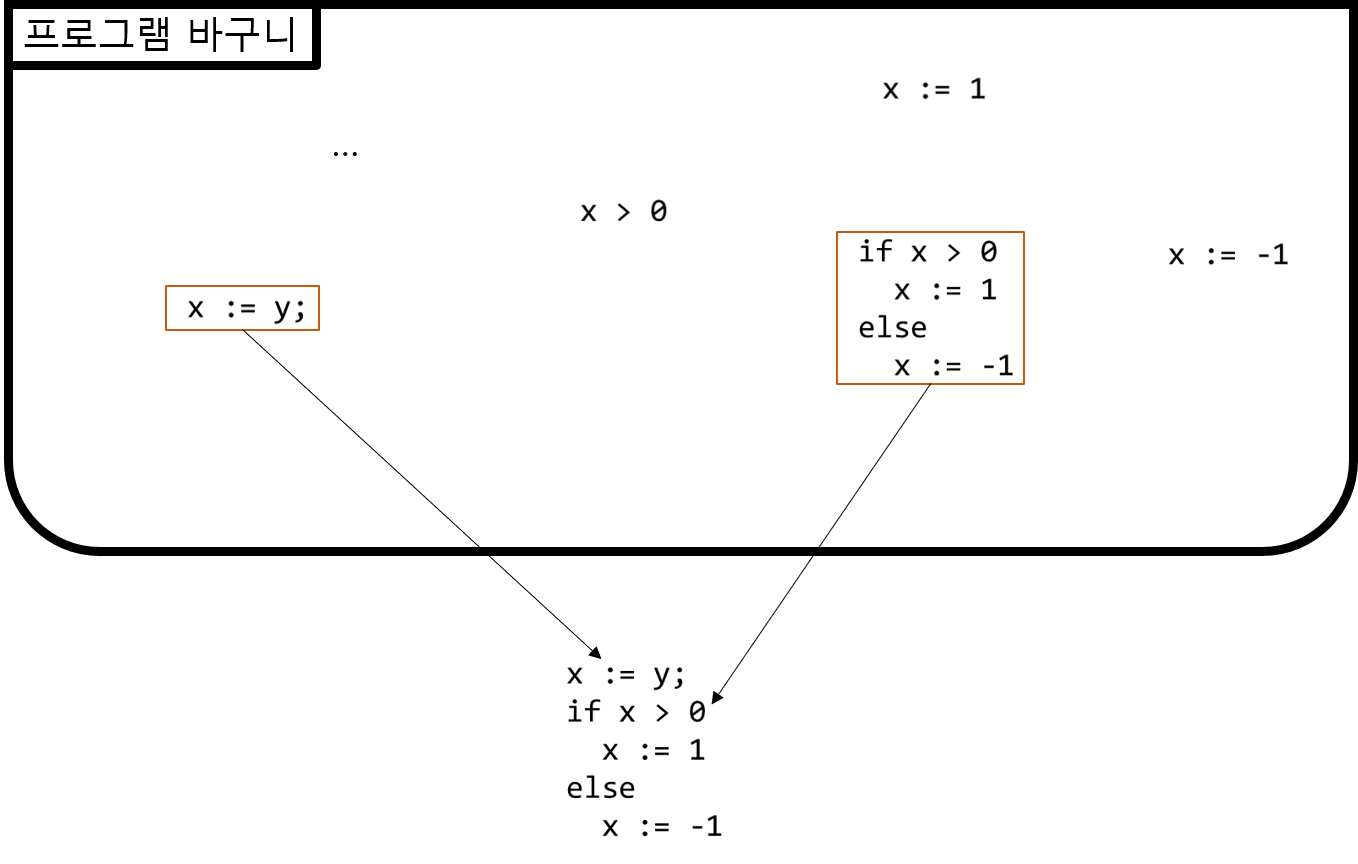
\includegraphics[width=0.9\textwidth]{img/prog4.png}}}%
    \only<2>{\noindent\makebox[\textwidth][c]{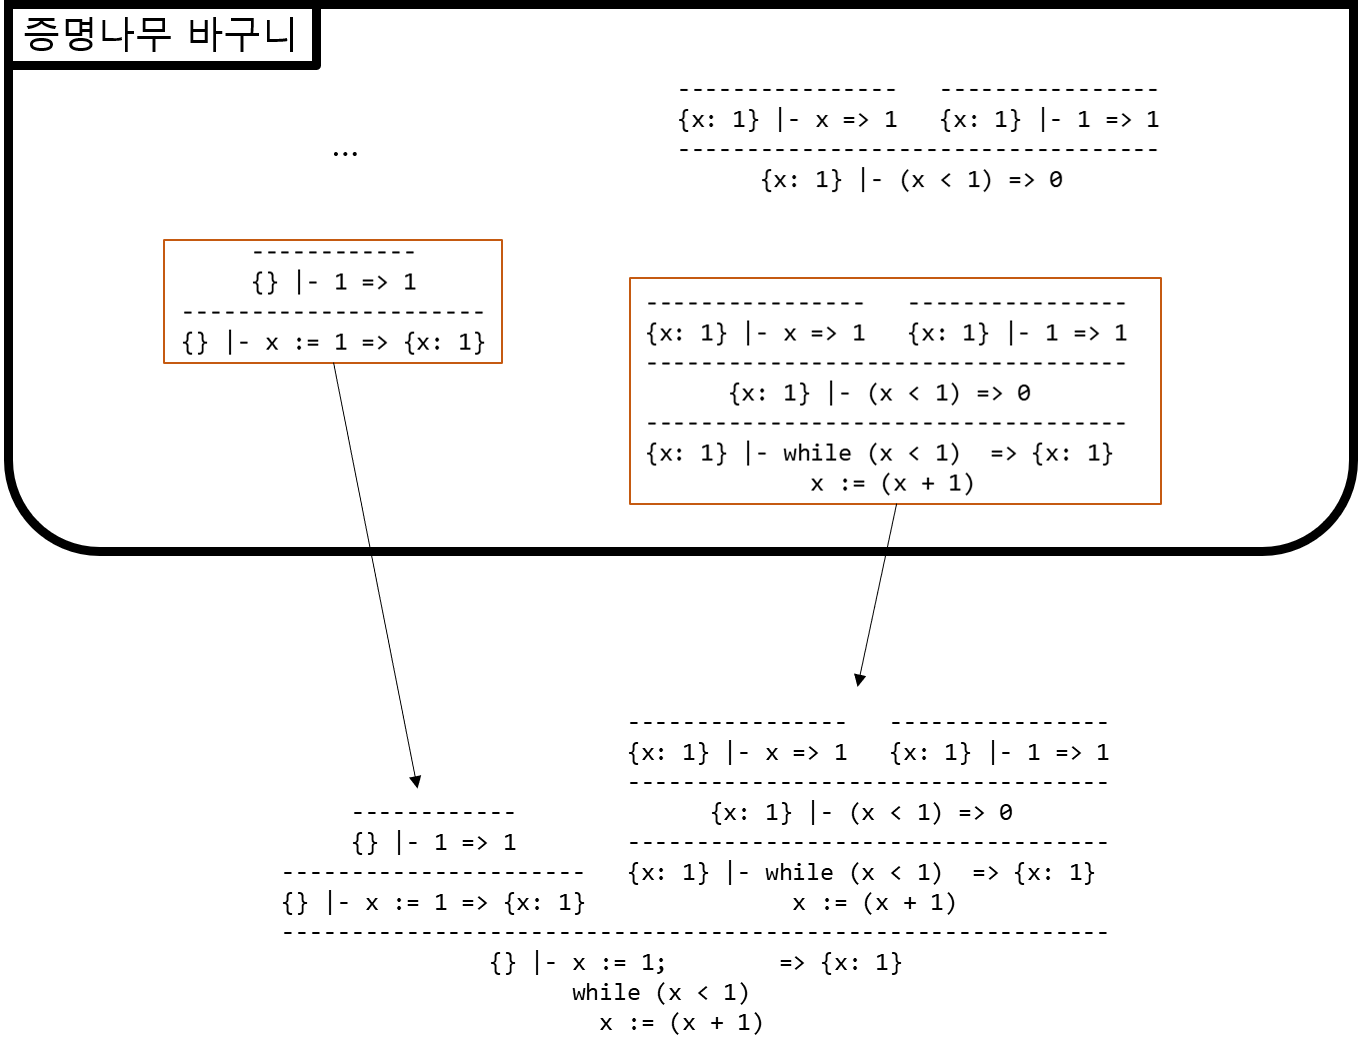
\includegraphics[width=0.9\textwidth]{img/proof4.png}}}%
  \end{overlayarea}

  \begin{itemize}
    \item<1-> 프로그램 합성 대신 증명나무 합성 방식을 사용
    \item<2-> 실행 의미가 존재하는 프로그램만을 뽑아내기 위함!
    \item<3-> 증명나무에는 항상 메모리가 따라 붙음
  \end{itemize}
\end{frame}

\begin{frame}
  \frametitle{메모리는 코드를 따라 자연스럽게 나오는 것이 아닌가?}
  \begin{itemize}
    \item<1-> 완전한 프로그램은 그 자체로 메모리를 결정할 수 있음
      \par\vspace{4pt}
      \hspace*{2.5em}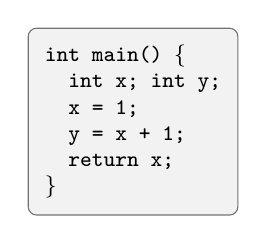
\begin{tikzpicture}
        \node[draw=black!55, rounded corners=3pt, fill=black!5, align=left,
              font=\ttfamily\footnotesize, inner sep=6pt] {%
          int main() \{\\
          \ \ int x; int y;\\
          \ \ x = 1;\\
          \ \ y = x + 1;\\
          \ \ return x;\\
          \}};
      \end{tikzpicture}
    \item<2-> 반면 부분 프로그램은 앞뒤 메모리의 \emph{관계}만 알 수 있음
      \par\vspace{6pt}
      \hspace*{2.5em}(전 메모리)\quad$\to$\quad\tikz[baseline=-0.6ex]{\node[draw=black!55, rounded corners=3pt, fill=black!5, font=\ttfamily\footnotesize, inner sep=6pt]{y = x + 1;};}\quad$\to$\quad(후 메모리)
  \end{itemize}
\end{frame}


\begin{frame}
  \frametitle{메모리를 최대한 나중에 결정하려고 하면...}
  \begin{center}
  \begin{tikzpicture}[
      treebox/.style={draw=black!25, rounded corners=2pt, inner sep=1pt},
      treecap/.style={font=\small},
      arr/.style={-{Stealth[length=3mm]}, very thick, black},
    ]
    \useasboundingbox (-4.9,-4.25) rectangle (5.05,1.3);
    % --- 위: 두 증명나무 (임시 그림, fig/ 아래 파일 교체) ---
    \node<1->[treebox] (t1) at (-3.1,0) {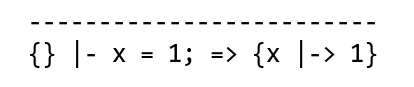
\includegraphics[width=3.3cm]{img/core_x_assign}};
    \node<1->[treecap, above=2pt of t1] {\texttt{x = 1;} 증명나무};
    \node<2->[treebox] (t2) at (2.0,0) {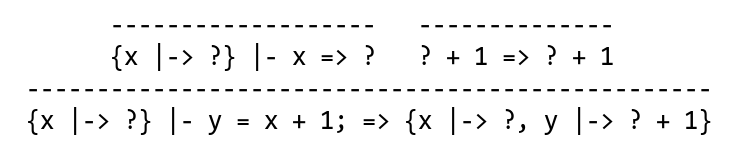
\includegraphics[width=5.9cm]{img/core_y_assign}};
    \node<2->[treecap, above=2pt of t2] {\texttt{y = x + 1;} 증명나무};
    % --- 아래: 합친 증명나무 ---
    \node<3->[treebox] (tc) at (0,-2.9) {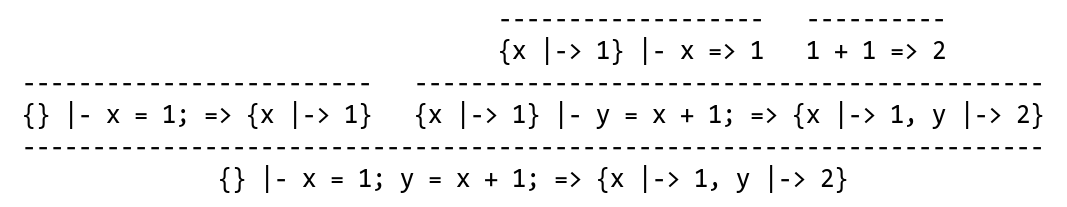
\includegraphics[width=9.6cm]{img/core_sequence_xy}};
    \node<3->[treecap, below=2pt of tc] {합친 증명나무};
    % --- 화살표 (합칠 때 등장) ---
    \draw<3->[arr] (t1.south) -- ([xshift=-1.8cm]tc.north);
    \draw<3->[arr] (t2.south) -- ([xshift=1.8cm]tc.north);
  \end{tikzpicture}
  \end{center}
  \uncover<4->{\begin{center}\textcolor{red}{어 되나?}\end{center}}
\end{frame}



\begin{frame}
  \frametitle{하지만 조건문, 반복문을 만나면...}
  \uncover<1->{
    \begin{center}
    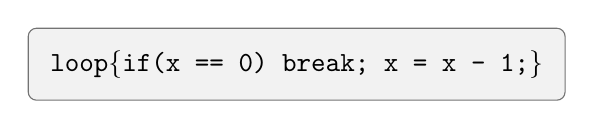
\begin{tikzpicture}[
        codeblock/.style={draw=black!55, rounded corners=3pt, fill=black!5,
          align=left, font=\ttfamily\normalsize, inner sep=8pt},
      ]
      \node[codeblock] {loop\{if(x == 0) break; x = x - 1;\}};
    \end{tikzpicture}
    \end{center}

    메모리를 모른 채로, 이 부분 프로그램의 증명나무를 그릴 수 있을까?
  }
  \uncover<2->{
    \begin{center}
    \small $x = 1$일 때\\[0.2em]
    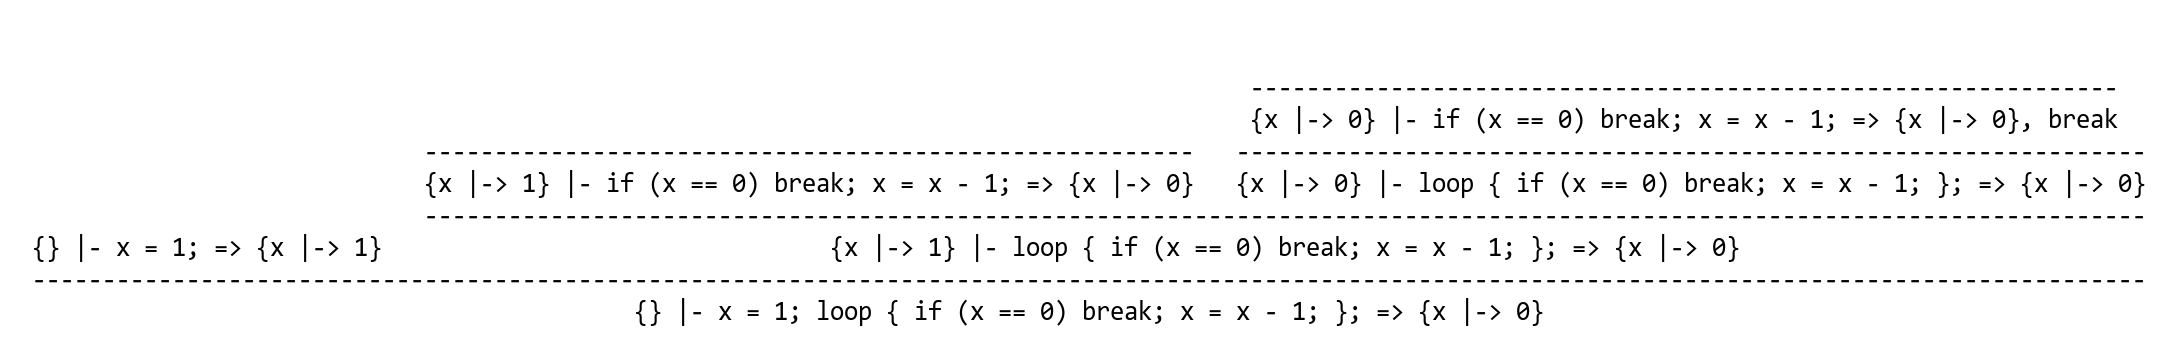
\includegraphics[scale=0.12]{img/x1loop.png}\\[0.6em]
  }
  \uncover<3->{
    \small $x = 2$일 때\\[0.2em]
    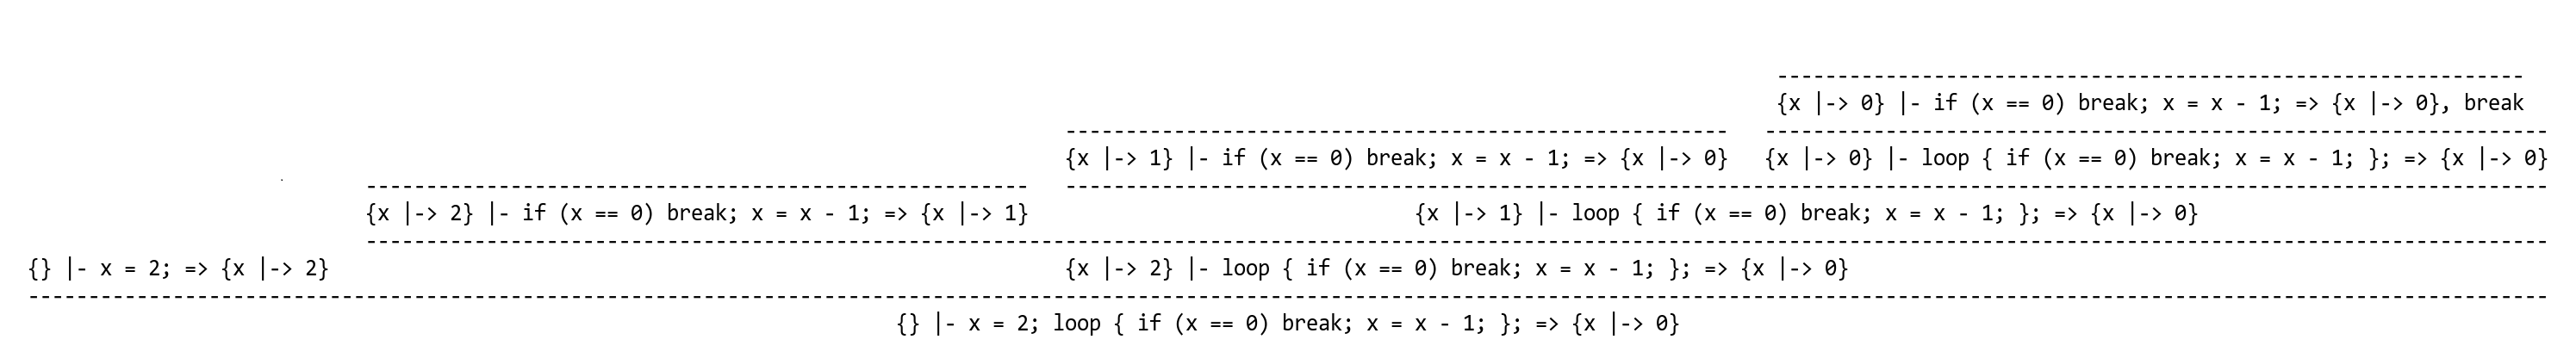
\includegraphics[scale=0.12]{img/x2loop.png}
    \end{center}
  }
  \uncover<4->{
    조립이 잘 안 됨!
  }
\end{frame}

\begin{frame}
  \frametitle{하지만 조건문, 반복문을 만나면...}

  \begin{itemize}
    \item<1-> 메모리를 후처리를 한다고 해도 무한히 돌거나 정지 문제를 해결해야 하는 딜레마에 빠짐.
    \item<2-> 따라서 메모리는 나중에 계산하면 안 되고, 작은 증명나무를 만들 때 전후 메모리가 확실하게 정해져야 함.
  \end{itemize}
\end{frame}

\begin{frame}[t]
  \frametitle{합성 시 메모리 관리}
  \begin{itemize}
    \item<1-> 실제 C 언어에서는 주소 연산을 통해 인접한 메모리를 마구 참조 가능하다.
    \item<2-> 특히 struct를 보면 적당히 포인터 + 1 연산을 이용해 인접 변수에 접근 가능.
    \item<3-> CIL, 혹은 \CILmm{}에서는 모든 변수가 외딴섬으로 존재해, 직접 그 변수를 통하지 않으면 해당 메모리 위치를 참조할 수 없게 한다. (포인터 제외)
    \item<4-> 따라서 어느 정도는 $\{x \mapsto 1,\ y \mapsto 2\}$ 이런 구조로 메모리를 생각할 수 있다.
  \end{itemize}
  \only<2>{%
    \AddToShipoutPictureFG*{%
      \put(\LenToUnit{0.5\paperwidth},\LenToUnit{0.30\paperheight}){\makebox(0,0){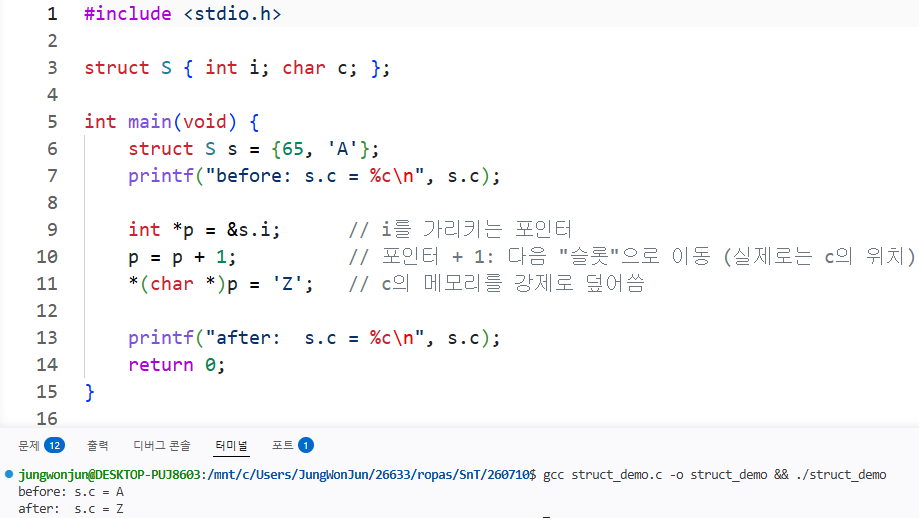
\includegraphics[width=0.7\textwidth]{img/struct-memory-hack.png}}}%
    }%
  }
\end{frame}

\begin{frame}
  \frametitle{stack frame 관리}
  \begin{itemize}
    \item<1-> 메모리에는 크게 heap, stack, global/static이 있다.
    \item<2-> 이 중 일단 stack만 보기로 하자. 다음 간단한 함수를 보자.
  \end{itemize}

  \uncover<2->{
    \begin{center}
    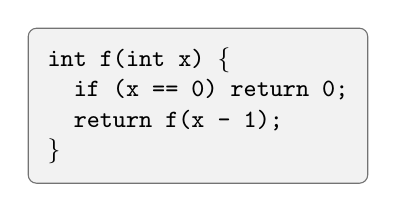
\begin{tikzpicture}[
        codeblock/.style={draw=black!55, rounded corners=3pt, fill=black!5,
          align=left, font=\ttfamily\small, inner sep=7pt},
      ]
      \node[codeblock] {%
        int f(int x) \{\\
        \ \ if (x == 0) return 0;\\
        \ \ return f(x - 1);\\
        \}
      };
    \end{tikzpicture}
    \end{center}
  }

  \begin{itemize}
    \item<3-> main에서 f(2)를 호출했을 때의 증명나무를 생각해 보자.
  \end{itemize}
\end{frame}


\begin{frame}[t]
  \frametitle{그렇지만 모든 frame을 보기엔 너무 크다}

  \begin{itemize}
    \item<1-> 마지막 f(0)이 호출되었을 때, 메모리 상태는 다음과 같다.
  \end{itemize}

  \uncover<1->{
    \begin{center}
    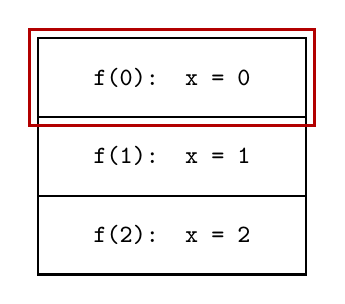
\begin{tikzpicture}[
        frame/.style={draw=none, fill=none,
          minimum width=3.4cm, minimum height=1cm, font=\ttfamily\small},
      ]
      \node[frame] (f2) at (0,0.5) {f(2): x = 2};
      \node[frame] (f1) at (0,1.5) {f(1): x = 1};
      \node[frame] (f0) at (0,2.5) {f(0): x = 0};
      \draw[black, thick] (-1.7,0) rectangle (1.7,3);
      \draw[black, thick] (-1.7,1) -- (1.7,1);
      \draw[black, thick] (-1.7,2) -- (1.7,2);
      \uncover<2->{
        \draw[red!70!black, very thick]
          ($(f0.north west)+(-3pt,3pt)$) rectangle ($(f0.south east)+(3pt,-3pt)$);
      }
    \end{tikzpicture}
    \end{center}
  }

  \begin{itemize}
    \item<2-> 그렇지만, 중요한(당장 봐야 하는)건 top frame뿐이다.
  \end{itemize}
\end{frame}

\begin{frame}
  \frametitle{그렇지만 모든 frame을 보기엔 너무 크다}

  \only<1>{
    \begin{center}%
      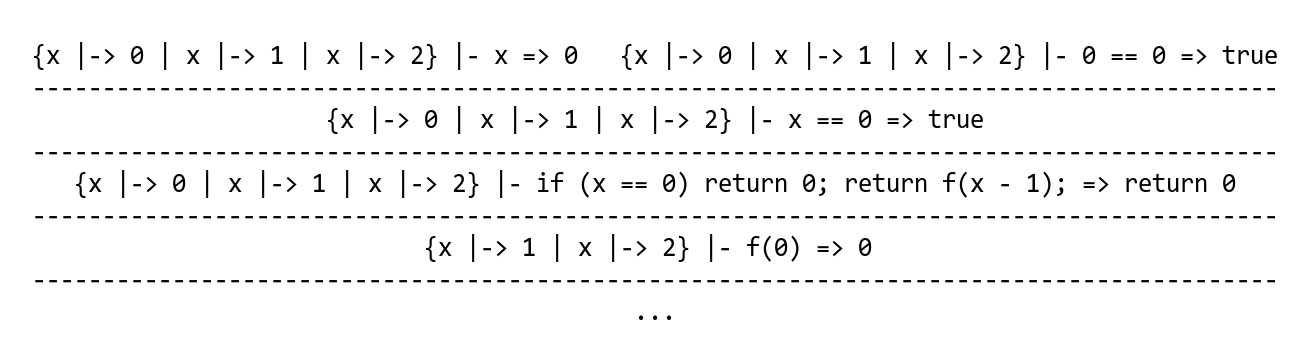
\includegraphics[scale = 0.3]{img/proof-tree-all-frames.png}\\[5pt]
      {\small 스택의 모든 프레임을 들고다니는 경우}%
    \end{center}
  }
  \only<2->{
    \begin{center}%
      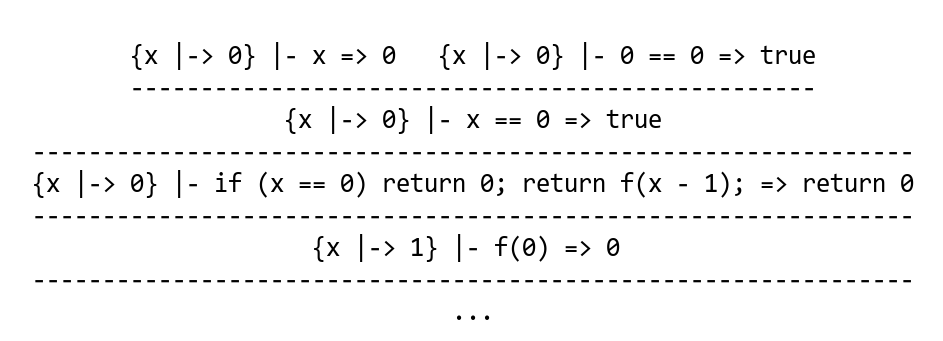
\includegraphics[scale = 0.3]{img/proof-tree-top-frame.png}\\[5pt]
      {\small top 프레임만 들고다니는 경우}%
    \end{center}
  }

  \begin{itemize}
    \item<3-> 포인터를 인자로 받으면 이전 frame에 간섭이 가능하지만, 그것도 결국 따로 접근 가능한 location으로 두고, 조립할때 location을 연결하면 된다.
  \end{itemize}
\end{frame}

\begin{frame}
  \frametitle{결국 메모리 관리는}
  \begin{itemize}
    \item<1-> 이제 합성에 필요한 메모리는 다시 $\{x \mapsto 1,\ y \mapsto 2\}$ 꼴이므로,
    \item<2-> (가능한 변수 이름(id) 목록, 가능한 값 목록)만 있으면 유한하게 메모리를 만들 수 있다.
    \item<3-> completeness 공격의 종료를 보장하기 위해서는 증명나무의 크기 증가와 함께 변수 이름, 가능한 값의 범위를 점차 넓혀가면 된다.
  \end{itemize}
\end{frame}

\section{앞으로 할 일}

\begin{frame}
  \frametitle{앞으로 할 일}

  \begin{itemize}
    \item<1-> 지금까지 한 일
      \begin{itemize}
        \item syntax, semantics(big-step), interpreter등 기본적인 것들 구현
      \end{itemize}
    \item<2-> 앞으로 할 일
      \begin{itemize}
        \item bottom-up 기반으로 합성 시작
        \item 각종 가지치기(pruning), 휴리스틱을 통한 시간 단축
        \item 실행 중 AI 가이드?
      \end{itemize}
    \item<3-> 걱정거리
      \begin{itemize}
        \item fibonacci.c만 해도 크기가 매우매우 큼.
        \item<5-> 재귀적으로 합성할 것/아닌 것을 구분해서 쉬운 step은 바로바로 진행되게끔 하는 전략이 필요할 듯
        \item<6-> 재귀호출에서의 program size 역전 문제 해결
      \end{itemize}
  \end{itemize}

  \only<4>{%
    \AddToShipoutPictureFG*{%
      \AtPageCenter{\makebox(0,0){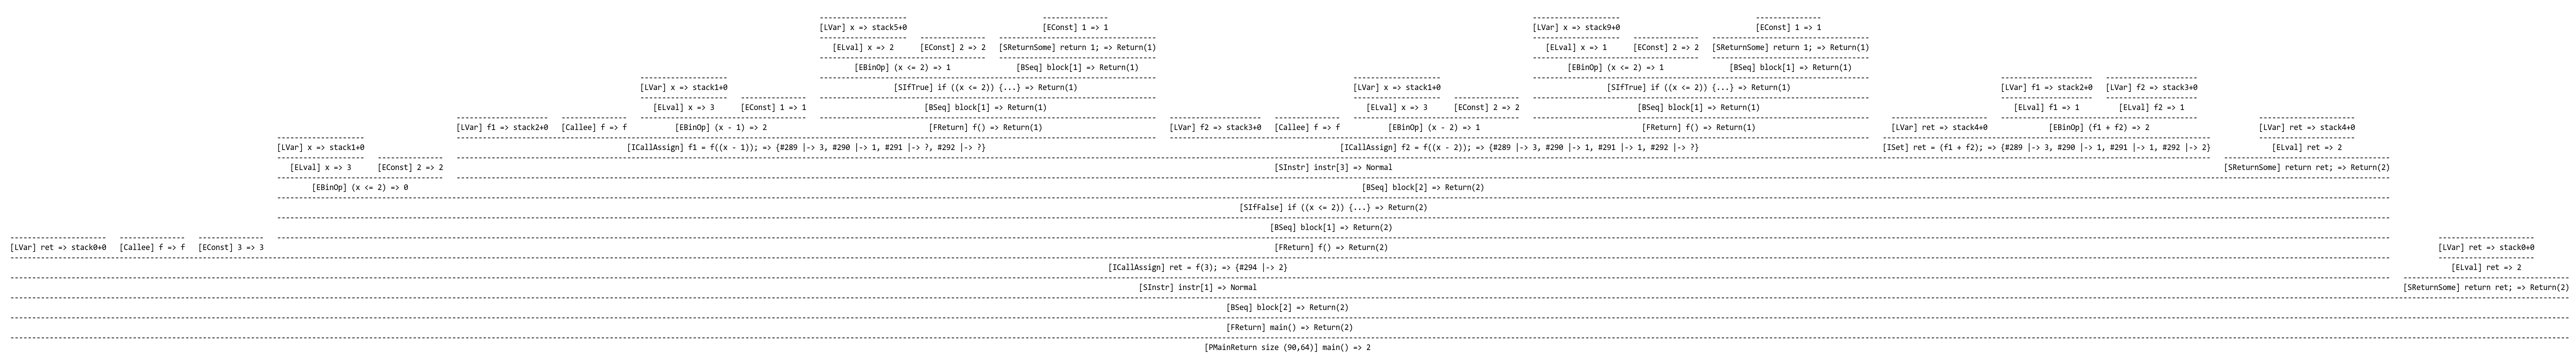
\includegraphics[scale=0.10]{img/fibonacci.png}}}%
    }%
  }
\end{frame}

\begin{frame}
  \frametitle{size 역전 현상}

  \begin{itemize}
    \item<1-> 원래 증명나무 합성은 (prog, proof) 크기 pair를 기준으로 작은 것부터 조립식으로 만들었음
      \begin{overlayarea}{\textwidth}{0.5\textheight}
        \only<1->{\noindent\makebox[\textwidth][c]{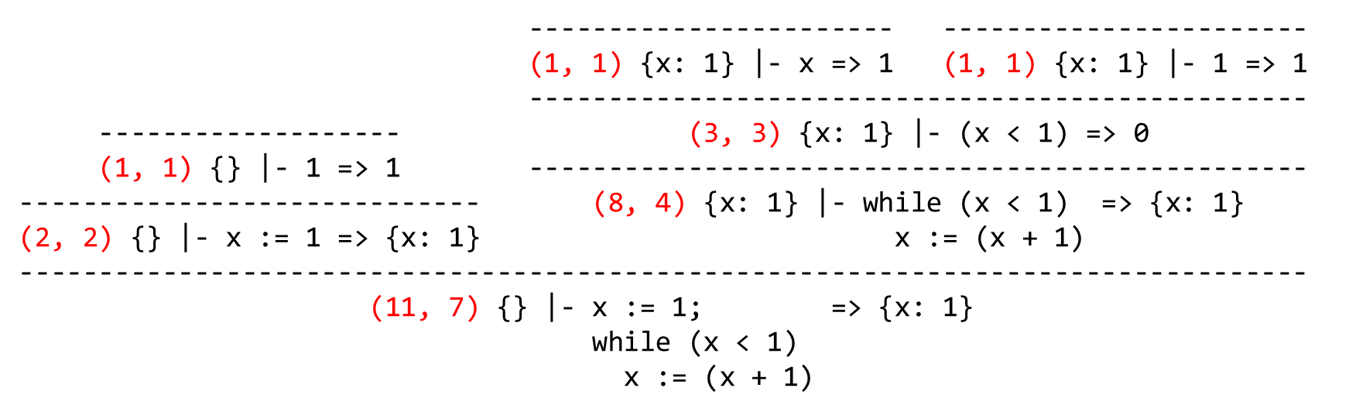
\includegraphics[width=0.9\textwidth,height=0.48\textheight,keepaspectratio]{img/pairsize.png}}}%
      \end{overlayarea}
    \item<2-> 크기 순서를 대각선($1,1 \rightarrow 2,1 \rightarrow 2,2 \rightarrow 3,1 \rightarrow \cdots$)으로 잡으면 모든 증명나무를 빠짐없이 탐색 가능
    \item<3-> 그런데, 함수 call을 하는 순간 부분나무가 전체 나무보다 크기가 커지는 문제가 발생!
  \end{itemize}

    % (prog_size, proof_size)로 했더니, 함수 call을 했더니 subtree가 prog_size가 더 커지는 문제가 발생
    % footprint 같은걸로 해도 여전히 이상함
    % prog_size를 왜 도입했는지를 생각해보자.
    % if() ``엄청 큰 코드'' 
    % 같은 데서 ``엄청 큰 코드''가 마구 생겨서 stuck되는 경우를 방지하기 위해서였다.
    % 이것만 해결하면 proof_size 순서만 사용해서 합성할 수 있지 않을까?
    % 그러면 엄청 큰 코드는 다 완성된 코드에만 추후에 붙이는 걸로 하면 되지 않을까? 오!
    % 생각해보니 실행 의미가 존재하는 프로그램만 합성하는건  P1 P2 ... 해서 한 스텝씩 실행시키는걸로도 가능하네? 대신 얘는 "빨리 하기" 기술이 적용이 잘 안 됨

\end{frame}



% 감사합니다

\definecolor{mydarkblue}{RGB}{32,56,61}

\setbeamercolor{background canvas}{bg=mydarkblue}
\setbeamercolor{normal text}{fg=white}
\setbeamercolor{frametitle}{fg=white}
\addtocounter{framenumber}{-1} % 마지막 슬라이드 번호를 하나 줄임
\appendix
\begin{frame}[c] % [c]는 내용 수직 가운데 정렬
  \centering
  {\Large \textcolor{white}{감사합니다}}
\end{frame}

\end{document}
